%*******************************************************************************
% Minute/Memorandum/Short Report Template - RSUQ / ETHZ
% This template is based on ETH minute
%
\documentclass[11pt]{article}

%*******************************************************************************
% ethminutes-config.tex
%
% Use it at the beginning of your ethMinutes.tex, or as a LaTeX Preamble 
% in your ethMinutes.{tex,lyx} with %*******************************************************************************
% ethminutes-config.tex
%
% Use it at the beginning of your ethMinutes.tex, or as a LaTeX Preamble 
% in your ethMinutes.{tex,lyx} with %*******************************************************************************
% ethminutes-config.tex
%
% Use it at the beginning of your ethMinutes.tex, or as a LaTeX Preamble 
% in your ethMinutes.{tex,lyx} with \input{ethminutes-config}
% ******************************************************************************  

%***********************
% 0. General information
%***********************
\NeedsTeXFormat{LaTeX2e}[1999/01/01]
\ProvidesPackage{ethminutes}[2013/21/01]

%*******************************************************************************
% 1. Set the encoding of your files.
% UTF-8 is the only sensible encoding nowadays.
% If you can't read ���������?���?�?,
% then change the encoding setting in your editor, not the line below.
% Make sure your editor supports UTF-8
%*******************************************************************************
\PassOptionsToPackage{latin1}{inputenc}
\usepackage{inputenc}
\PassOptionsToPackage{T1}{fontenc} % T2A for cyrillics
\usepackage{fontenc} 
\UseRawInputEncoding

%******************************************
% 2. Languages and other special characters
%******************************************
\usepackage[english]{babel}               % For adopting the typographical rules for French
\usepackage{eurosym}

%\usepackage{rawfonts}                    % 
%\usepackage{charter}                     %
%\usepackage[charter]{mathdesign}         %

%******************************************
% 3. Packages for color, image, and picture
%******************************************
\usepackage{xcolor}     % For color printing
\usepackage{graphicx}   % For flexible insertion and greater control of graphics
\usepackage{colortbl}	  % For putting color into table
\usepackage{tikz}       %
\usepackage{subfigure}  % For 
\usepackage{rotate}     % For rotation 

%***************
% 3. Setup table
%***************
\usepackage{booktabs}
\usepackage{tabularx}     
\newcolumntype{Y}{>{\centering\arraybackslash}X}
\newcommand{\lratio}[1]{\setlength{\hsize}{#1\hsize}}
\usepackage{multirow}

%****************
% 4. Bibliography 
%****************
\usepackage{hyperref}   % Inline hyperlink
%\usepackage{natbib}     % Bibliography using Author-year format
\usepackage[backend=bibtex,bibencoding=ascii,style=numeric,sorting=none,doi=false]{biblatex}
\addbibresource{../../outReachEmail/scopusBibTeX20180803-4.bib}

%******************
% 5. Other packages
%******************
\usepackage{fancyhdr}
\usepackage{ifthen}       % Add if/then/else command for LaTeX
\usepackage{ulem}         % Flexible command for underline
\normalem
\usepackage{bstnotations} % Notations table from Phimeca

%**********************
% Load the minute style
%**********************
\usepackage{ethminutes} 

\endinput
% ******************************************************************************  

%***********************
% 0. General information
%***********************
\NeedsTeXFormat{LaTeX2e}[1999/01/01]
\ProvidesPackage{ethminutes}[2013/21/01]

%*******************************************************************************
% 1. Set the encoding of your files.
% UTF-8 is the only sensible encoding nowadays.
% If you can't read ���������?���?�?,
% then change the encoding setting in your editor, not the line below.
% Make sure your editor supports UTF-8
%*******************************************************************************
\PassOptionsToPackage{latin1}{inputenc}
\usepackage{inputenc}
\PassOptionsToPackage{T1}{fontenc} % T2A for cyrillics
\usepackage{fontenc} 
\UseRawInputEncoding

%******************************************
% 2. Languages and other special characters
%******************************************
\usepackage[english]{babel}               % For adopting the typographical rules for French
\usepackage{eurosym}

%\usepackage{rawfonts}                    % 
%\usepackage{charter}                     %
%\usepackage[charter]{mathdesign}         %

%******************************************
% 3. Packages for color, image, and picture
%******************************************
\usepackage{xcolor}     % For color printing
\usepackage{graphicx}   % For flexible insertion and greater control of graphics
\usepackage{colortbl}	  % For putting color into table
\usepackage{tikz}       %
\usepackage{subfigure}  % For 
\usepackage{rotate}     % For rotation 

%***************
% 3. Setup table
%***************
\usepackage{booktabs}
\usepackage{tabularx}     
\newcolumntype{Y}{>{\centering\arraybackslash}X}
\newcommand{\lratio}[1]{\setlength{\hsize}{#1\hsize}}
\usepackage{multirow}

%****************
% 4. Bibliography 
%****************
\usepackage{hyperref}   % Inline hyperlink
%\usepackage{natbib}     % Bibliography using Author-year format
\usepackage[backend=bibtex,bibencoding=ascii,style=numeric,sorting=none,doi=false]{biblatex}
\addbibresource{../../outReachEmail/scopusBibTeX20180803-4.bib}

%******************
% 5. Other packages
%******************
\usepackage{fancyhdr}
\usepackage{ifthen}       % Add if/then/else command for LaTeX
\usepackage{ulem}         % Flexible command for underline
\normalem
\usepackage{bstnotations} % Notations table from Phimeca

%**********************
% Load the minute style
%**********************
\usepackage{ethminutes} 

\endinput
% ******************************************************************************  

%***********************
% 0. General information
%***********************
\NeedsTeXFormat{LaTeX2e}[1999/01/01]
\ProvidesPackage{ethminutes}[2013/21/01]

%*******************************************************************************
% 1. Set the encoding of your files.
% UTF-8 is the only sensible encoding nowadays.
% If you can't read ���������?���?�?,
% then change the encoding setting in your editor, not the line below.
% Make sure your editor supports UTF-8
%*******************************************************************************
\PassOptionsToPackage{latin1}{inputenc}
\usepackage{inputenc}
\PassOptionsToPackage{T1}{fontenc} % T2A for cyrillics
\usepackage{fontenc} 
\UseRawInputEncoding

%******************************************
% 2. Languages and other special characters
%******************************************
\usepackage[english]{babel}               % For adopting the typographical rules for French
\usepackage{eurosym}

%\usepackage{rawfonts}                    % 
%\usepackage{charter}                     %
%\usepackage[charter]{mathdesign}         %

%******************************************
% 3. Packages for color, image, and picture
%******************************************
\usepackage{xcolor}     % For color printing
\usepackage{graphicx}   % For flexible insertion and greater control of graphics
\usepackage{colortbl}	  % For putting color into table
\usepackage{tikz}       %
\usepackage{subfigure}  % For 
\usepackage{rotate}     % For rotation 

%***************
% 3. Setup table
%***************
\usepackage{booktabs}
\usepackage{tabularx}     
\newcolumntype{Y}{>{\centering\arraybackslash}X}
\newcommand{\lratio}[1]{\setlength{\hsize}{#1\hsize}}
\usepackage{multirow}

%****************
% 4. Bibliography 
%****************
\usepackage{hyperref}   % Inline hyperlink
%\usepackage{natbib}     % Bibliography using Author-year format
\usepackage[backend=bibtex,bibencoding=ascii,style=numeric,sorting=none,doi=false]{biblatex}
\addbibresource{../../outReachEmail/scopusBibTeX20180803-4.bib}

%******************
% 5. Other packages
%******************
\usepackage{fancyhdr}
\usepackage{ifthen}       % Add if/then/else command for LaTeX
\usepackage{ulem}         % Flexible command for underline
\normalem
\usepackage{bstnotations} % Notations table from Phimeca

%**********************
% Load the minute style
%**********************
\usepackage{ethminutes} 

\endinput


\selectlanguage{english}

%
\graphicspath{{./},{./figures/}}
\renewcommand{\baselinestretch}{1.3}

%********************
% Document properties
%******************** 
\RefDocument{\uqlab~External Citations (Q2/2018)}
\Date{03.08.2018}
\Redacteur{D. Wicaksono}     
\TitleReport{\uqlab~External Citations (Q2/2018)}
\DateDiffusion{August 3, 2018}
\From{D. Wicaksono}
\To{B. Sudret \& S. Marelli}
\CC{\uqlab~Devs.}

%**************
% Main document
%**************
\begin{document}

%====================
% Put the template on
%====================
\Header
\Footer 
\FrontPage

%===================
\section*{Summary}
%===================

As of 03.08.2018, a search in Scopus database for articles citing \uqlab~-- be they in journals, conference proceedings, or book series -- results in $81$ hits.
Out of that $81$ hits, $60$ do not list either Bruno nor Stefano as co-authors.
Finally, after additional skimming into each paper, $47$ articles that explicitly used \uqlab~in their research were identified, while the rest is simply citing that~\uqlab~is available as a tool.
Table~\ref{tab:citing_articles} lists the articles according to the identified scientific domains.
Tables~\ref{tab:citing_journals} and~\ref{tab:citing_conference} list the journal and conference proceeding names, respectively.
Finally, Fig.~\ref{fig:citing} illustrates the number of publications citing \uqlab~over time
and Fig.~\ref{fig:citing_tf} and~\ref{fig:citing_tfidf} compare the terms appeared in the abstracts between internal (including collaboration) and external articles.
\begin{table}[!ht]
    \centering
    \caption{\uqlab~domain of applications based on citing articles.}
    \label{tab:citing_articles} 
    \begin{tabularx}{0.75\textwidth}{cllX}\toprule
      \textbf{No.} & \textbf{Domain} & \textbf{Count} & \textbf{Citing Articles}\\\midrule        
      1           & electrical engineering                 &  13 & \cite{Barbi2018,Ni2018,Larbi2018a,Larbi2018,Larbi2017,Li2017,Larbi2017a,Du2017a,Du2017,Ni2017,Acikgoz2016,Bilicz2016,Bdour2016}\\
      2           & civil engineering                      &   8 & \cite{Fengjie2018,Dutta2018,Hariri-Ardebili2018,Chen2017,Mylonas2017a,Mylonas2017,Sanctis2016,Abdallah2016}\\
      3           & computational science and engineering  &   7 & \cite{Cheng2018,Palar2018,Palar2018a,Kaintura2017,Hashemian2017,Abraham2017,Abraham2016}
      \\
      4           & sensors engineering                    &   4 & \cite{Yuzugullu2017,Erten2016,Erten2016a,Capellari2016}\\
      5           & ocean engineering                      &   3 & \cite{Colone2018,Gaspar2016a,Gaspar2016} \\
      6           & geomechanics                           &   3 & \cite{Toe2018,Toe2017,Mentani2016}\\
      7           & chemical engineering                   &   3 & \cite{Xie2018,Xie2017,Schenkendorf2017}\\
      8           & nuclear engineering                    &   2 & \cite{Turati2018,Wu2018a}\\
      9           & biomedical science                     &   2 & \cite{Chiaramello2017,Perko2016}\\      
      10          & geoscience                             &   1 & \cite{Hamdi2017}\\
      11          & mechanical engineering                 &   1 & \cite{Vohra2018}\\
                  & \textbf{Total}                         &  47 & \\\bottomrule
  \end{tabularx}
\end{table}

\section{Introduction}

\begin{table}[!ht]
  \centering
  \caption{Journals with articles citing \uqlab.}
  \label{tab:citing_journals} 
  \begin{tabularx}{\textwidth}{cXc}\toprule
    \textbf{No.} & \textbf{Journal Name} & \textbf{Count} \\\midrule
1 & IEEE Transactions on Power Systems & 2\\
2 & Reliability Engineering and System Safety & 2\\
3 & IEEE Transactions on Electromagnetic Compatibility & 2\\
4 & Structural and Multidisciplinary Optimization & 1\\
5 & Archives of Civil and Mechanical Engineering & 1\\
6 & BioMed Research International & 1\\
7 & Computational Geosciences & 1\\
8 & Earthquake Engineering and Engineering Vibration & 1\\
9 & Engineering Optimization & 1\\
10 & Engineering with Computers & 1\\
11 & IEEE Antennas and Wireless Propagation Letters & 1\\
12 & IEEE Journal of Selected Topics in Applied Earth Observations and Remote Sensing & 1\\
13 & IFAC-PapersOnLine & 1\\
14 & Rock Mechanics and Rock Engineering & 1\\
15 & Journal of Computational Physics & 1\\
16 & Landslides & 1\\
17 & Ocean Engineering & 1\\
18 & Physics in Medicine and Biology & 1\\
19 & Progress in Electromagnetics Research & 1\\
20 & Progress in Nuclear Energy & 1\\
21 & Remote Sensing of Environment & 1\\
22 & Renewable Energy & 1\\
23 & Applied Mathematics and Computation & 1\\
24 & International Journal of Heat and Mass Transfer & 1\\\bottomrule
  \end{tabularx}
\end{table}

\begin{table}[!ht]
  \centering
  \caption{Conference proceedings or collections with articles citing \uqlab.}
  \label{tab:citing_conference} 
  \begin{tabularx}{\textwidth}{cXc}\toprule
    \textbf{No.} & \textbf{Proceedings} & \textbf{Count} \\\midrule
1 & ECCOMAS Congress 2016 - Proceedings of the 7th European Congress on Computational Methods in Applied Sciences and Engineering & 2\\
2 & Computer Aided Chemical Engineering & 2\\
3 & Proceedings of 3rd International Conference on Maritime Technology and Engineering, MARTECH 2016 & 2\\
4 & 2016 IEEE Wireless Power Transfer Conference, WPTC 2016 & 1\\
5 & 2017 11th European Conference on Antennas and Propagation, EUCAP 2017 & 1\\
6 & 2017 IEEE MTT-S International Conference on Numerical Electromagnetic and Multiphysics Modeling and Optimization for RF, Microwave, and Terahertz Applications, NEMO 2017 & 1\\
7 & 2017 IEEE Symposium Series on Computational Intelligence, SSCI 2017 - Proceedings & 1\\
8 & 2017 International Symposium on Electromagnetic Compatibility - EMC EUROPE 2017, EMC Europe 2017 & 1\\
9 & 2018 IEEE 22nd Workshop on Signal and Power Integrity, SPI 2018 - Proceedings & 1\\
10 & UNCECOMP 2017 - Proceedings of the 2nd International Conference on Uncertainty Quantification in Computational Sciences and Engineering & 1\\
11 & Proceedings of the 2017 19th International Conference on Electromagnetics in Advanced Applications, ICEAA 2017 & 1\\
12 & IABSE Conference, Vancouver 2017: Engineering the Future - Report & 1\\
13 & ICPE 2017 - Proceedings of the 2017 ACM/SPEC International Conference on Performance Engineering & 1\\
14 & International Geoscience and Remote Sensing Symposium (IGARSS) & 1\\
15 & Lecture Notes in Computer Science (including subseries Lecture Notes in Artificial Intelligence and Lecture Notes in Bioinformatics) & 1\\
16 & Procedia Engineering & 1\\
17 & 2016 IEEE Antennas and Propagation Society International Symposium, APSURSI 2016 - Proceedings & 1\\\bottomrule
  \end{tabularx}
\end{table}

\begin{figure}[!ht]
  \centering
  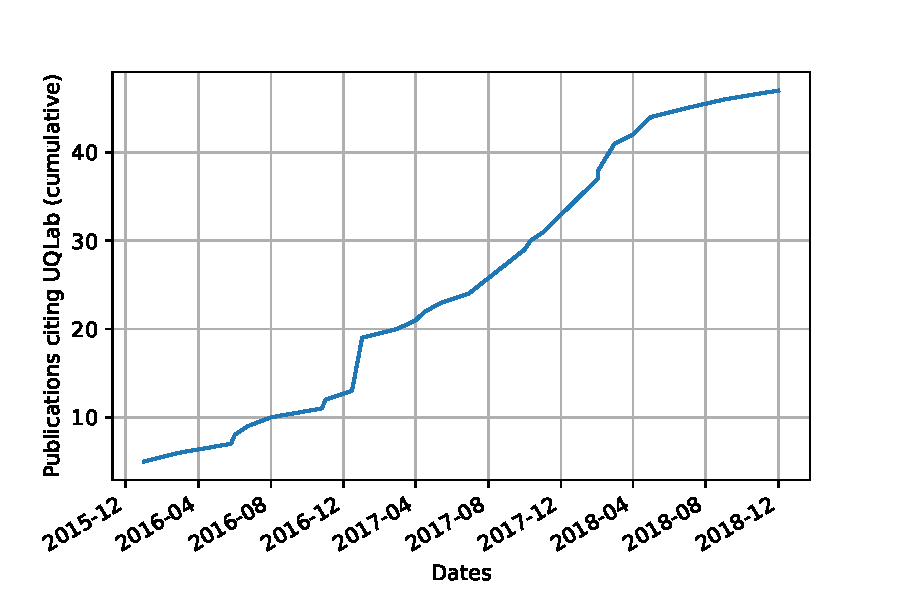
\includegraphics[width=0.8\textwidth]{citing.pdf}
  \caption{The number of publications citing \uqlab~over time.}
  \label{fig:citing}
\end{figure}


\begin{figure}
\centering     %%% not \center
\subfigure[Internal and collaborations ($21$ articles)]{\label{fig:citing_internal_tf}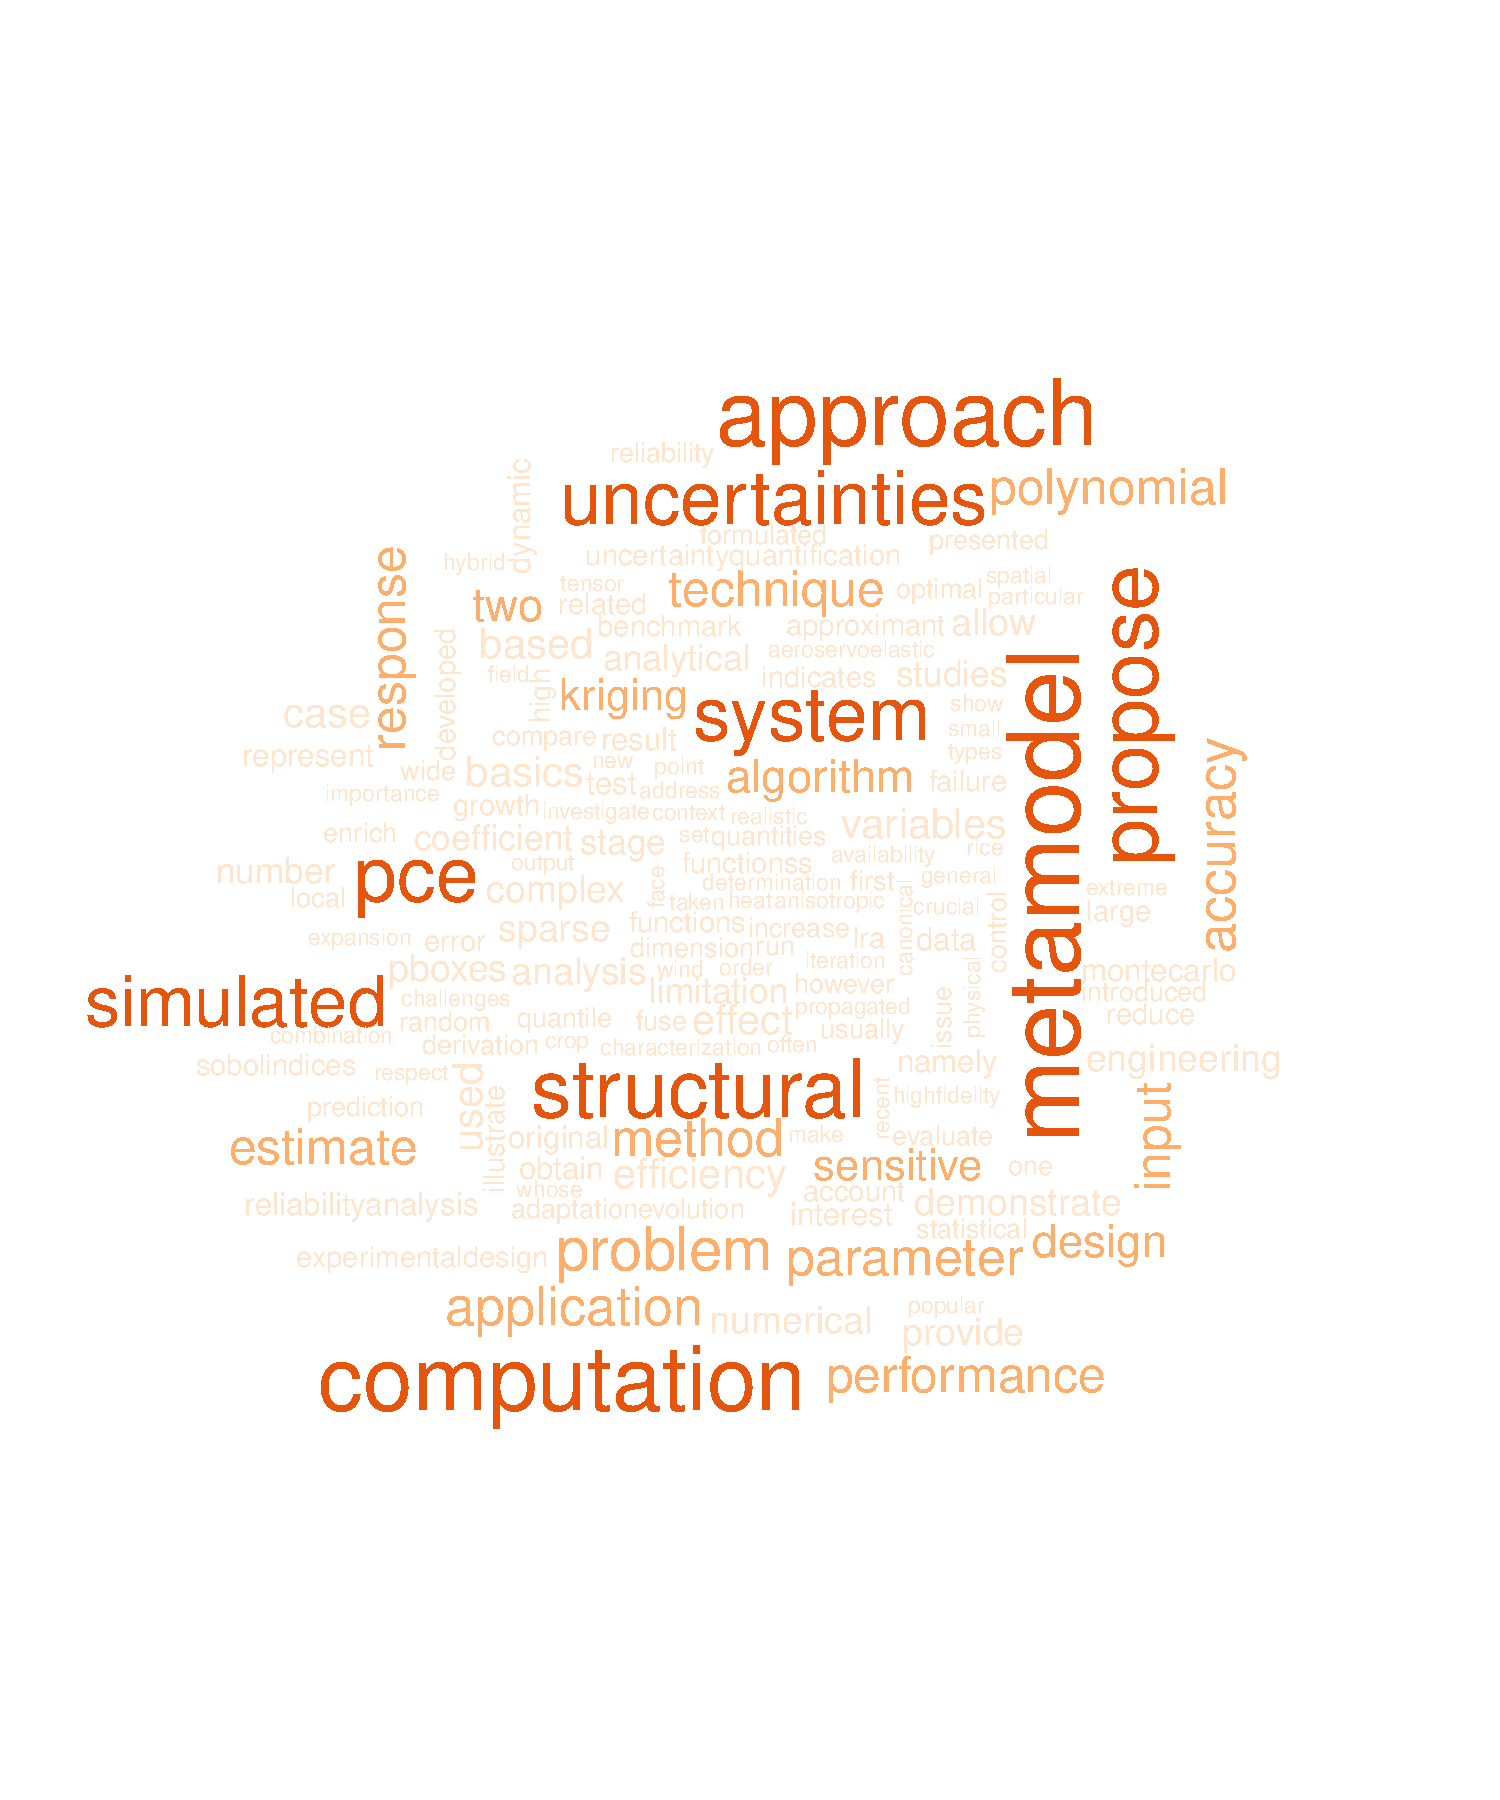
\includegraphics[width=0.45\textwidth]{wordcloud_internal_tf.pdf}}
\subfigure[External ($47$ articles)]{\label{fig:citing_external_tf}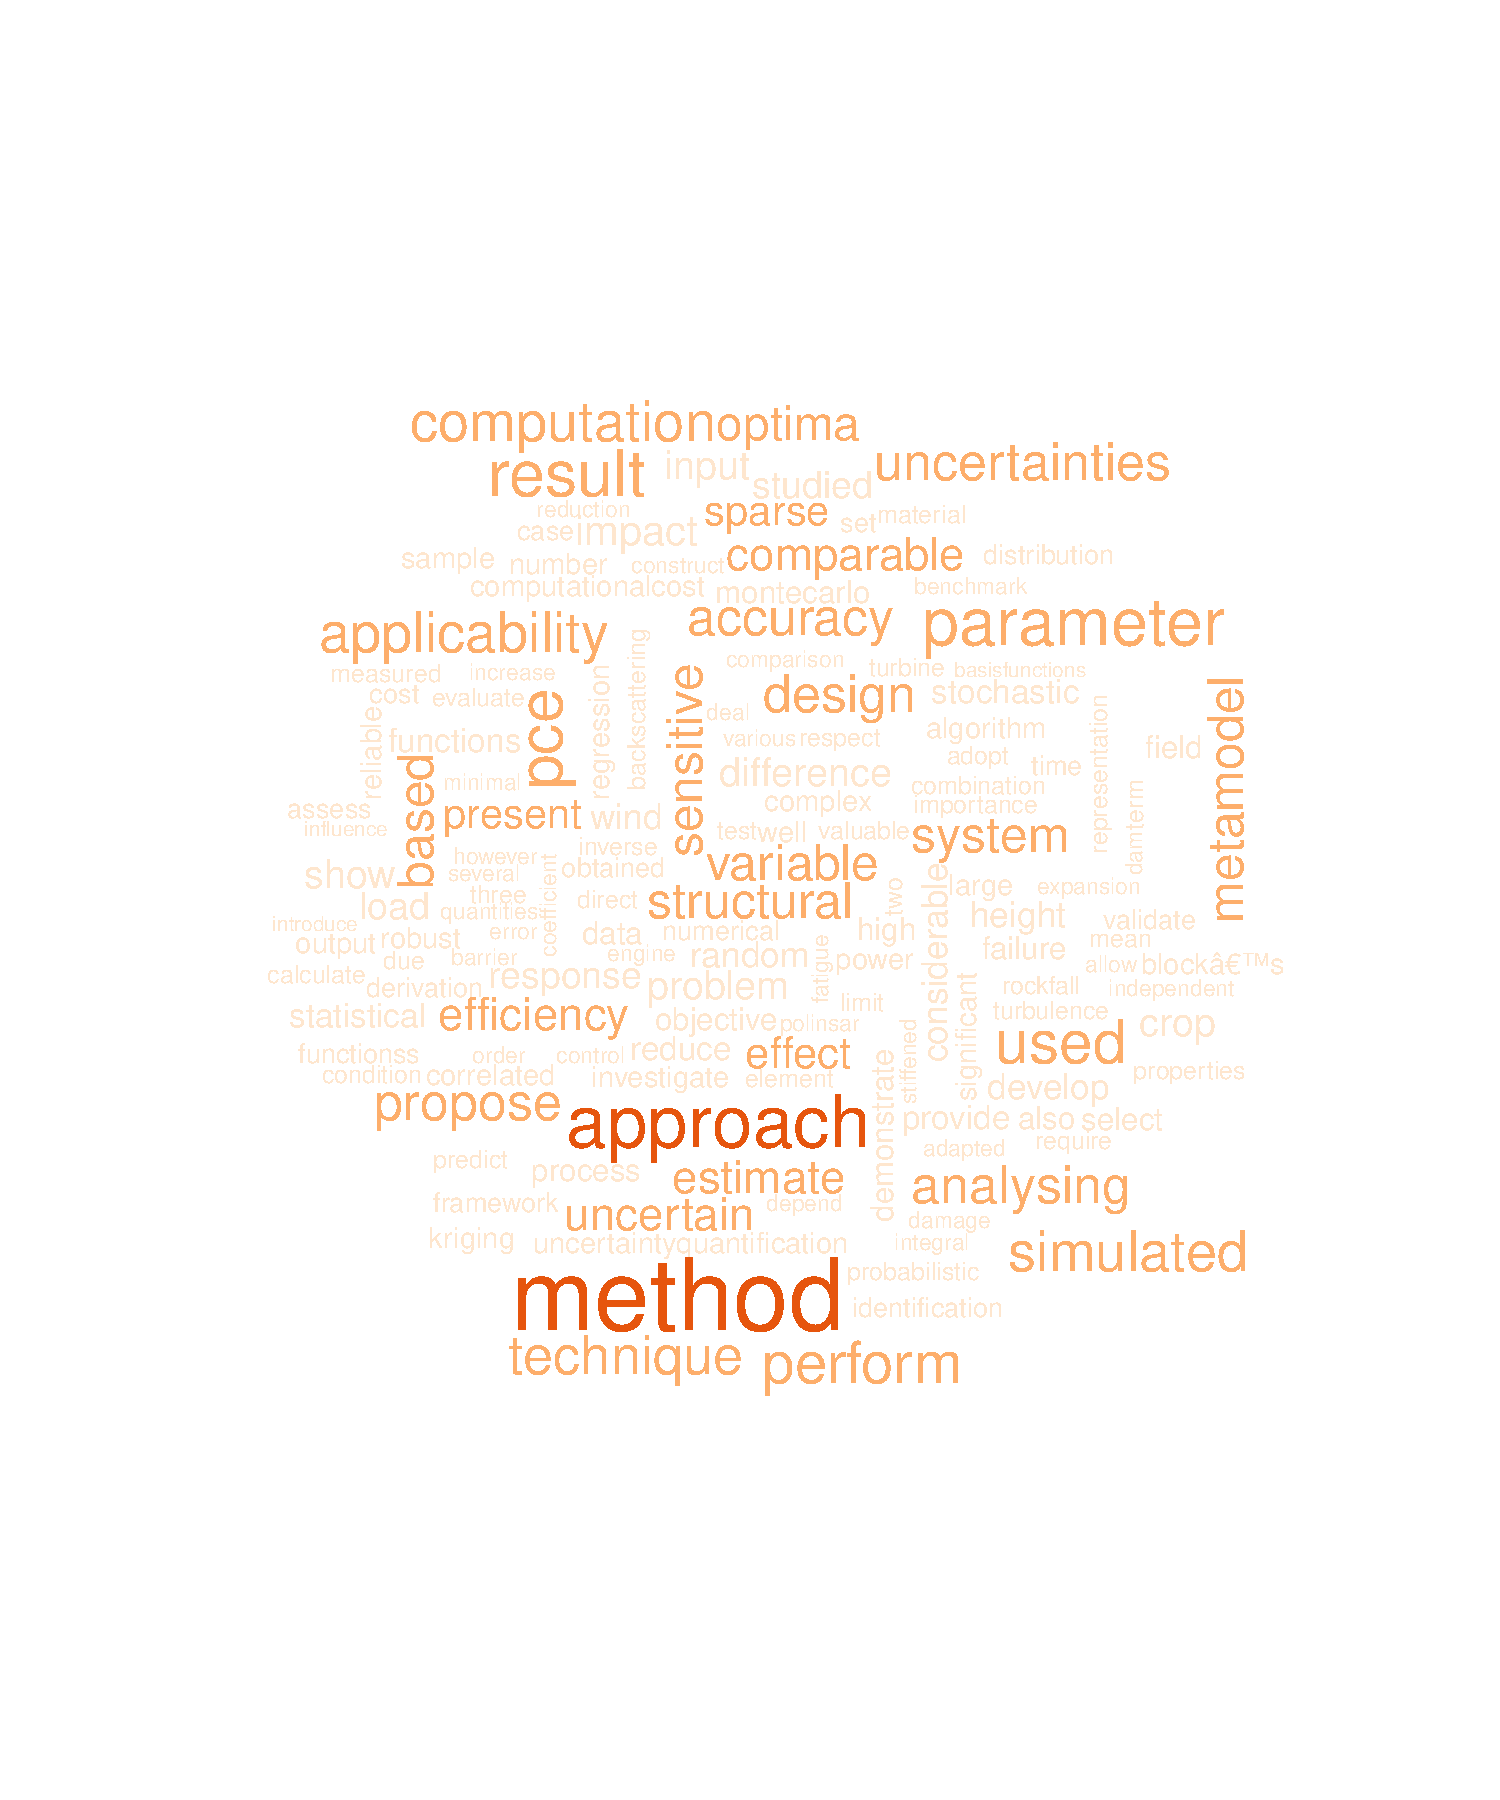
\includegraphics[width=0.45\textwidth]{wordcloud_external_tf.pdf}}
\caption{Word clouds of popular terms appeared in the abstract of articles citing \uqlab~weighted by TF (\emph{Term Frequency}). Using TF, the clouds display the most used terms in a collection of documents. Larger terms mean that the terms appear more across documents.}
\label{fig:citing_tf}
\end{figure}

\begin{figure}
\centering     %%% not \center
\subfigure[Internal and collaborations ($21$ articles)]{\label{fig:citing_internal_tfidf}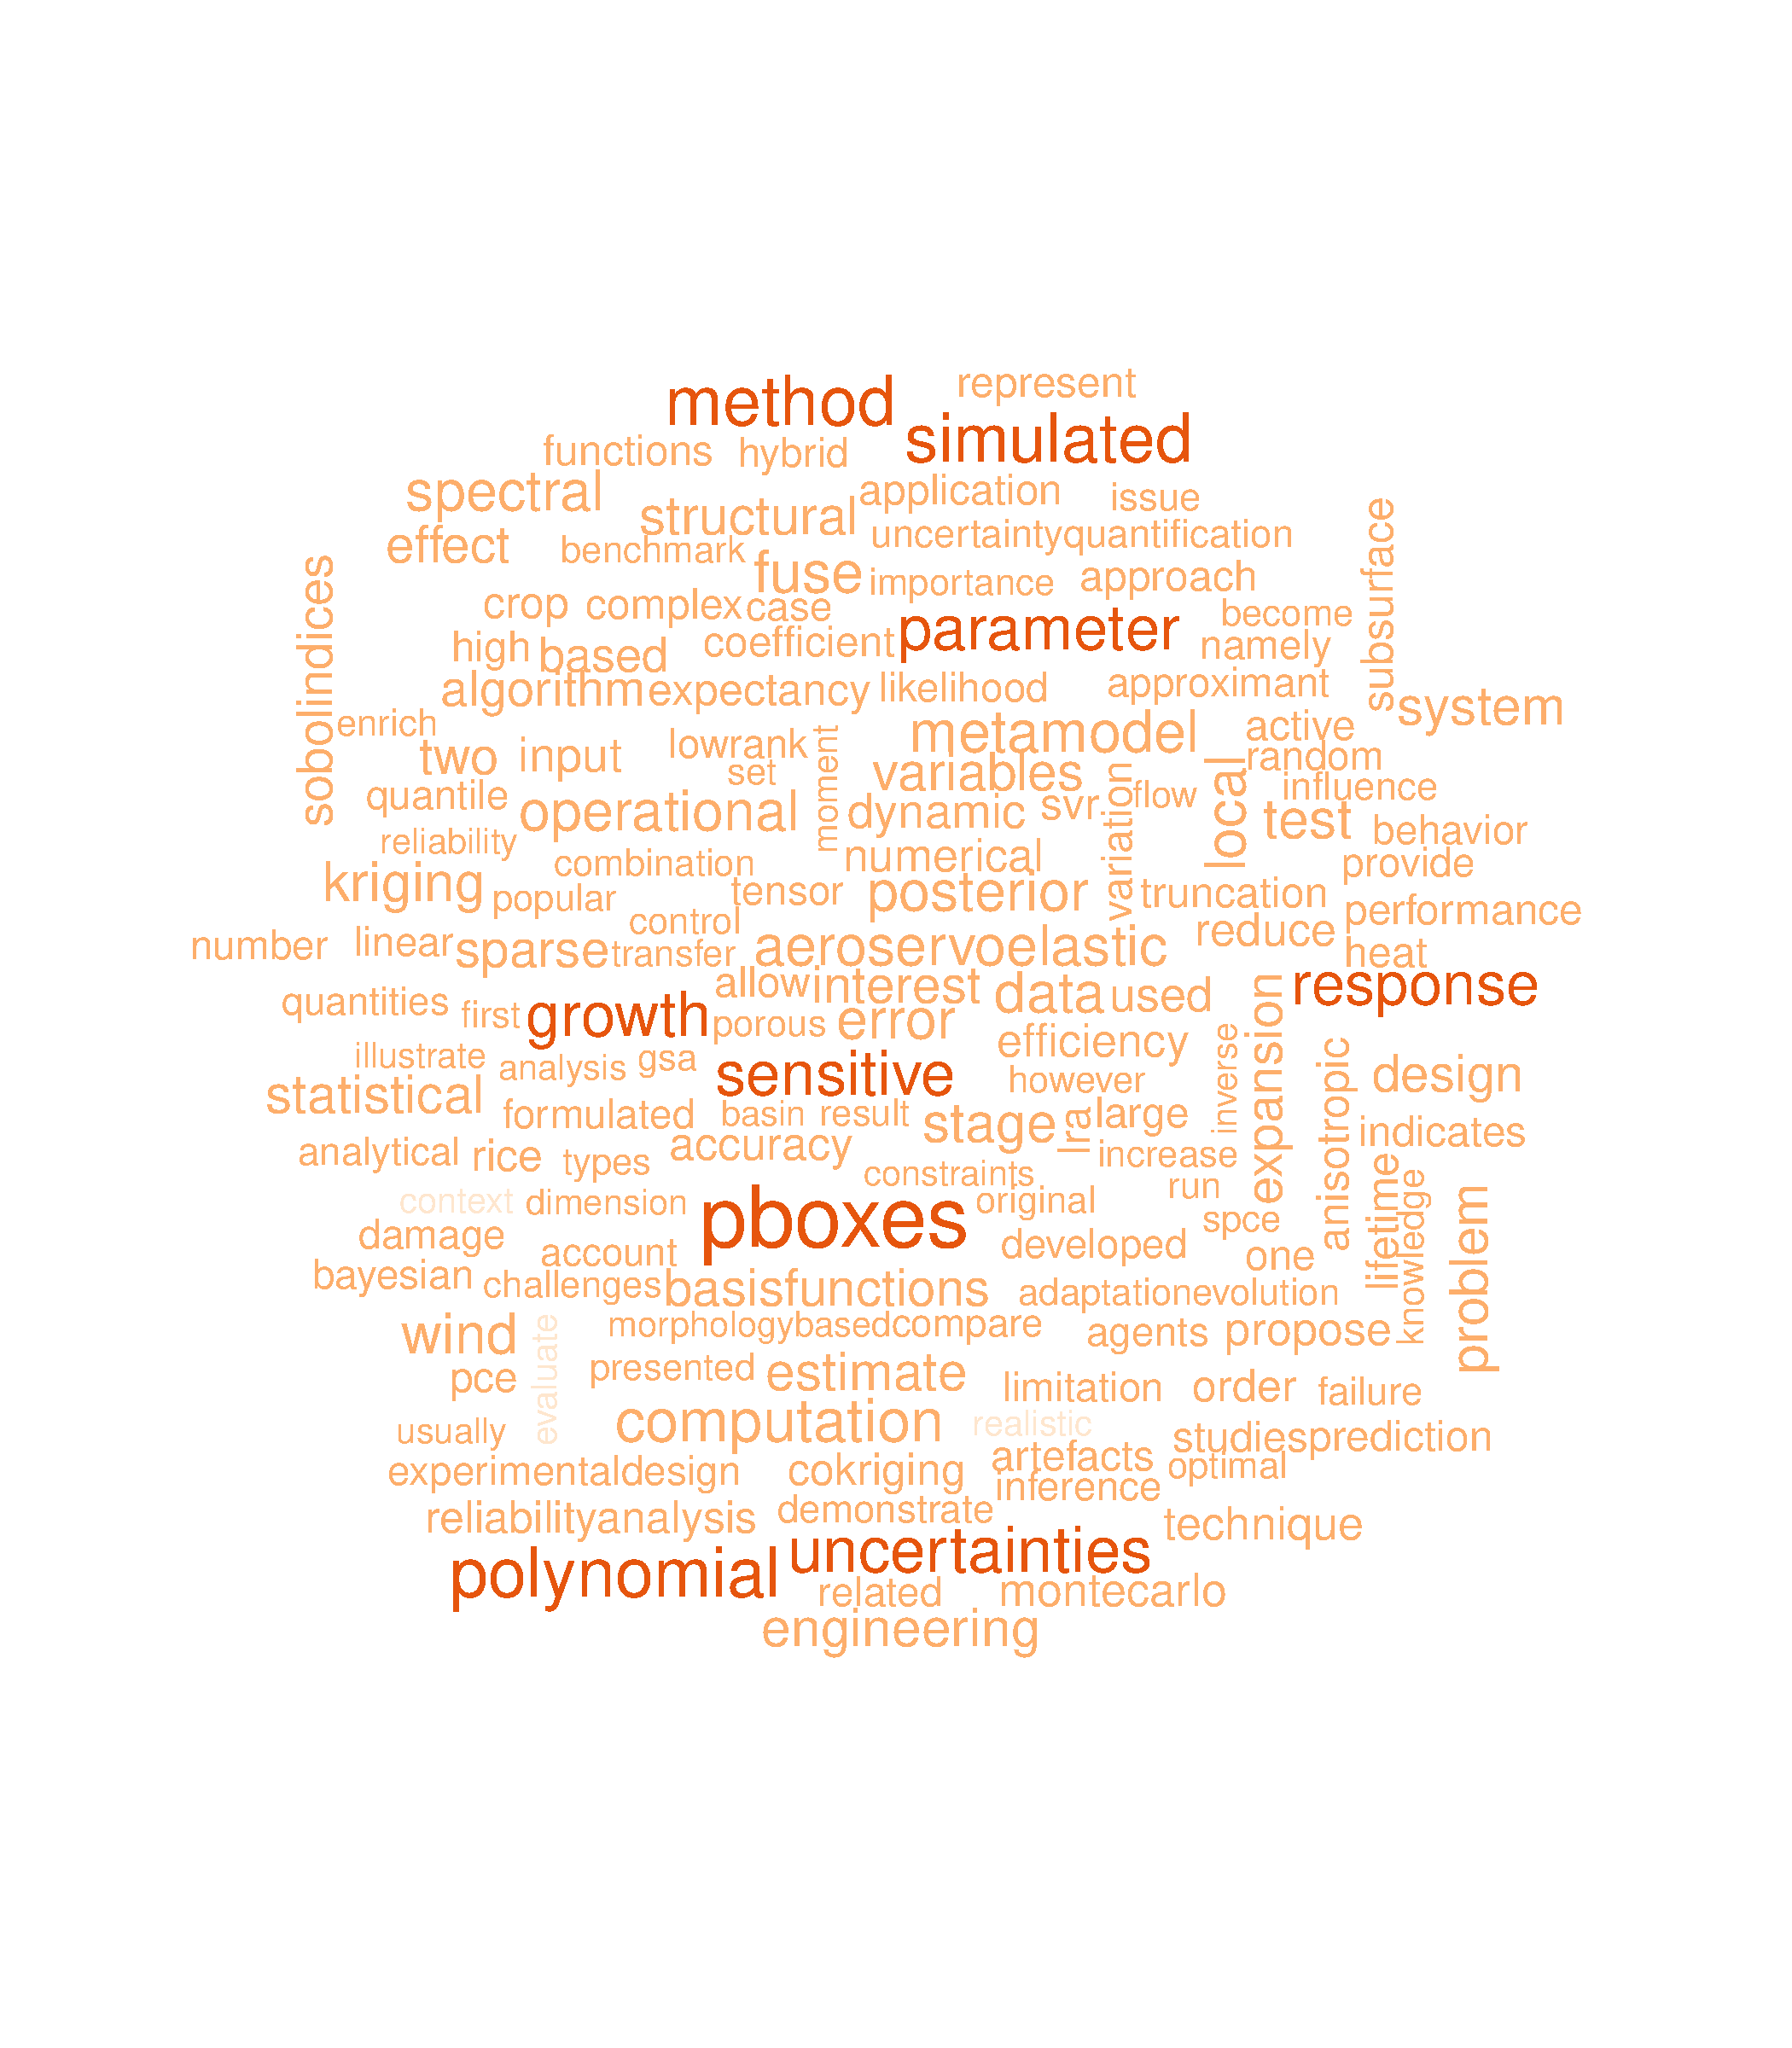
\includegraphics[width=0.45\textwidth]{wordcloud_internal_tfidf.pdf}}
\subfigure[External ($47$ articles)]{\label{fig:citing_external_tfidf}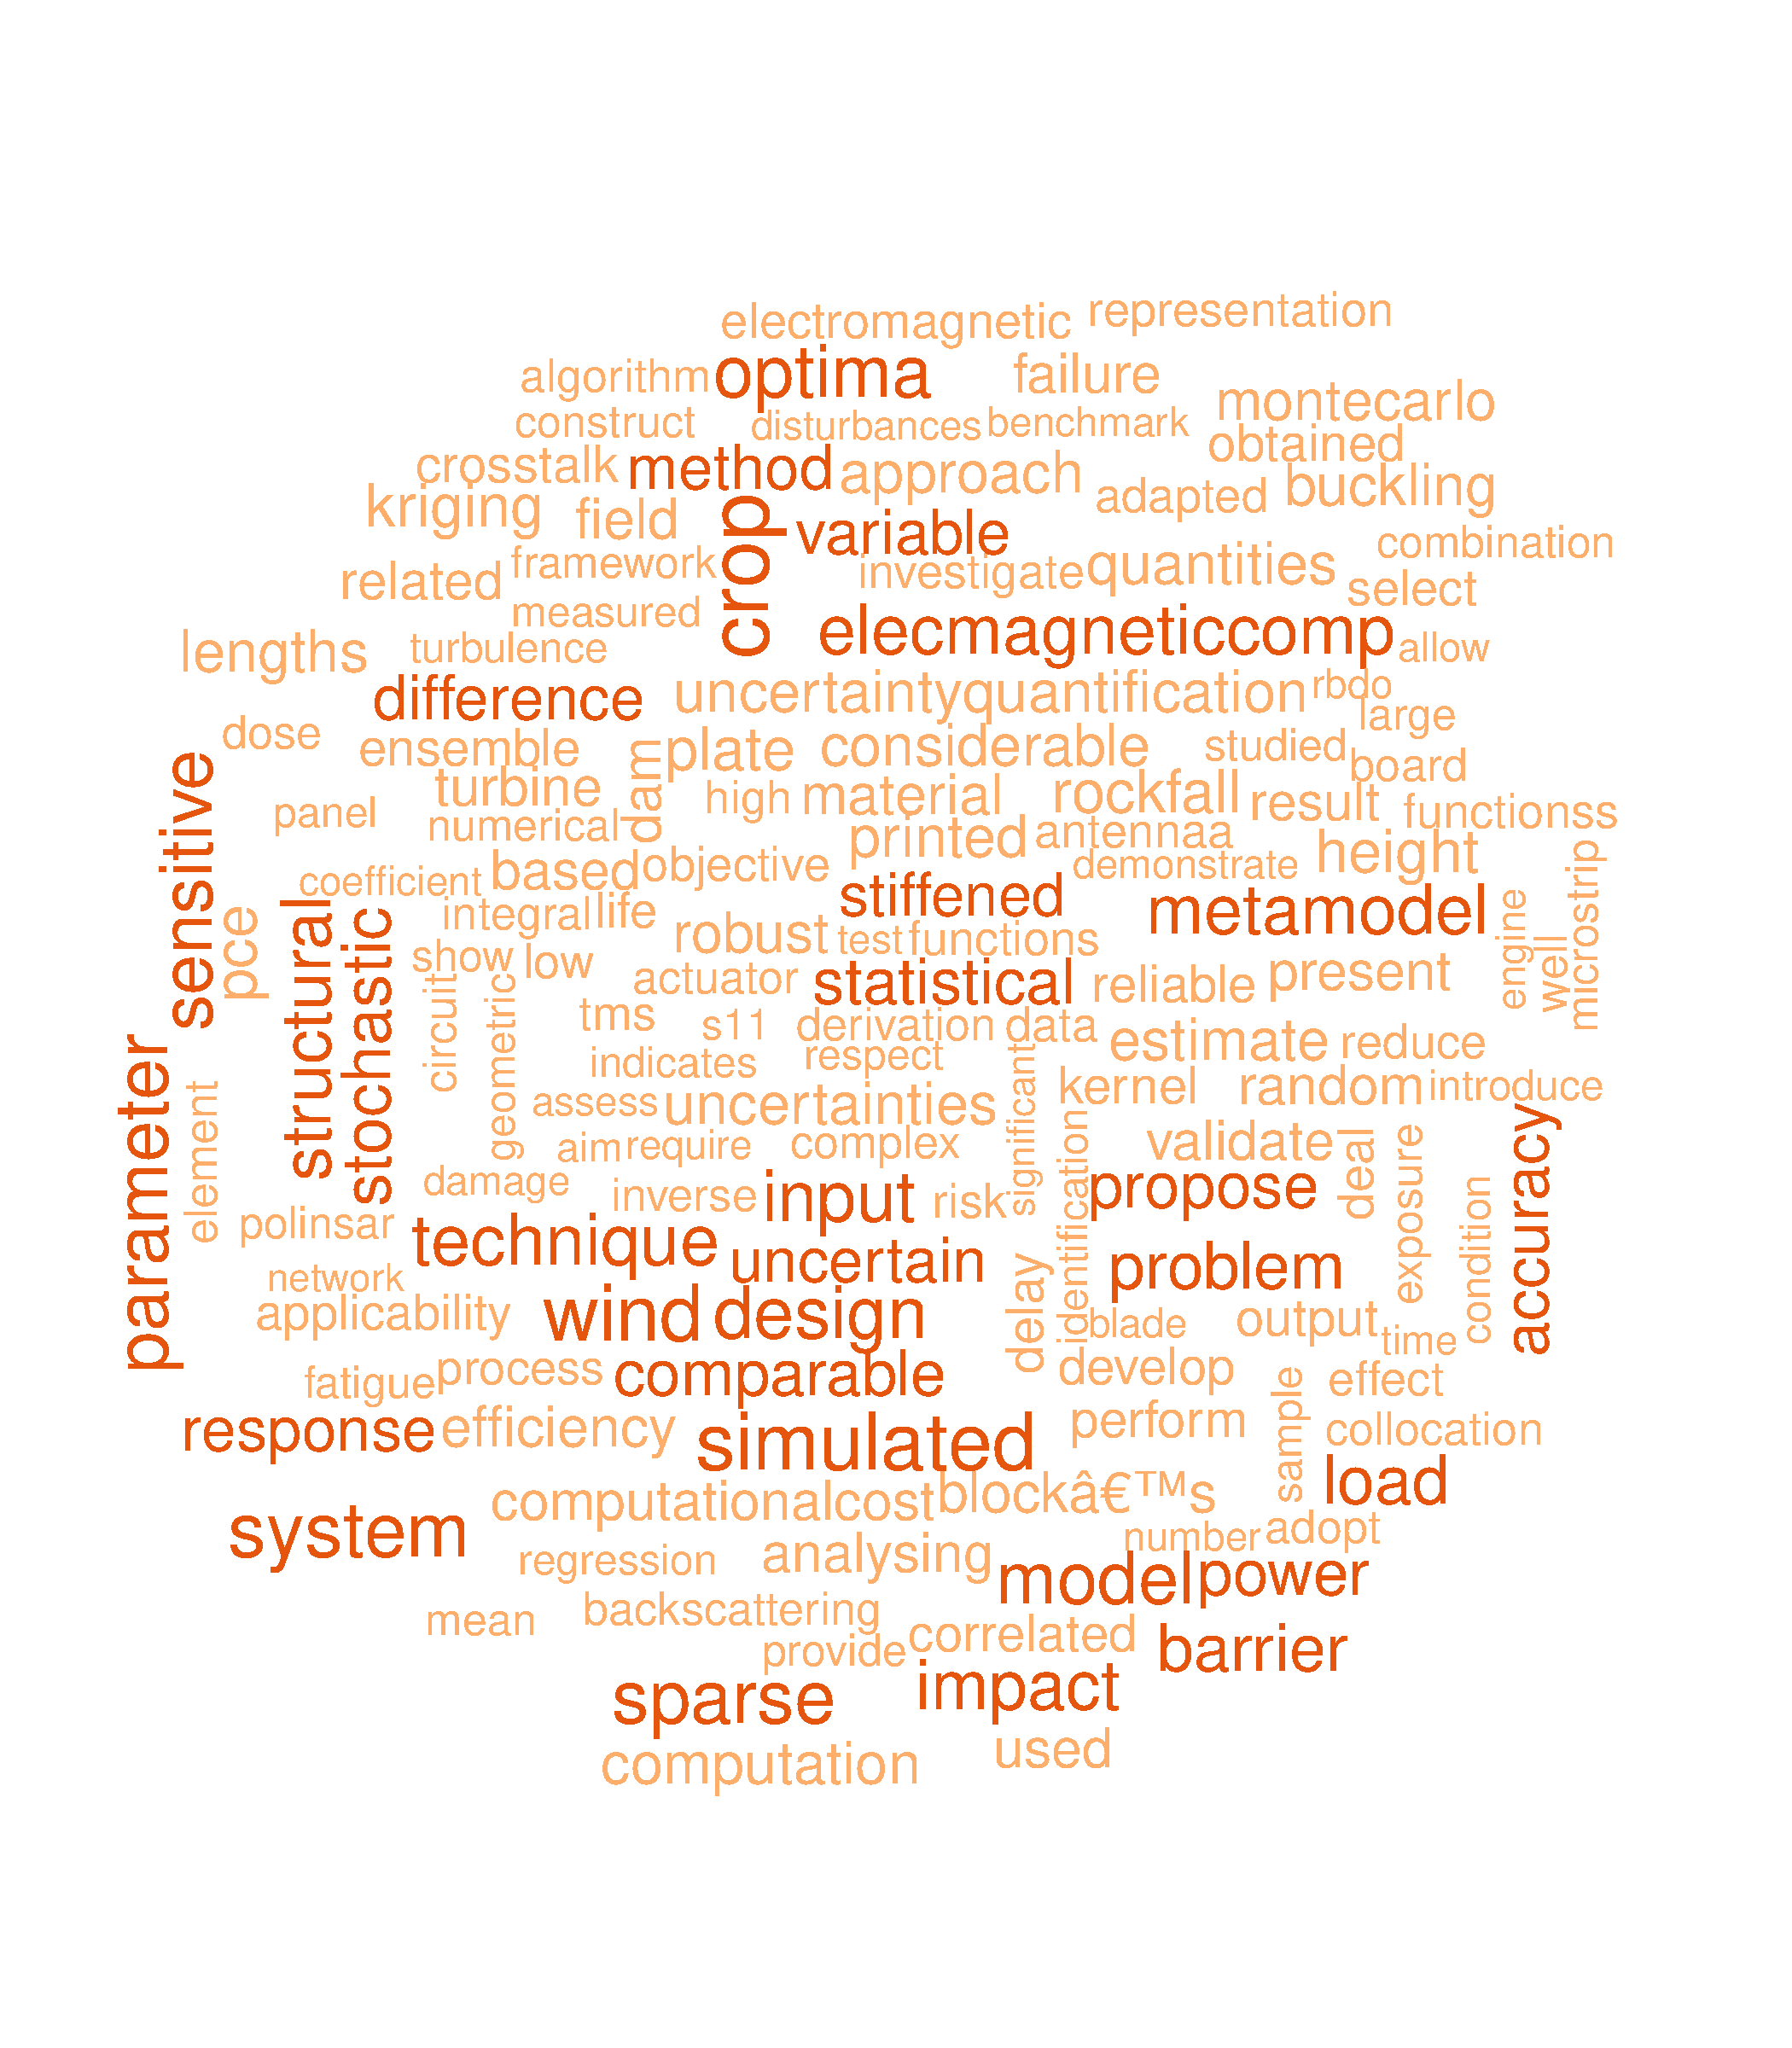
\includegraphics[width=0.45\textwidth]{wordcloud_external_tfidf.pdf}}
\caption{Word clouds of unique terms appeard in the abstract of articles citing \uqlab~weighted by TF-IDF (\emph{Term Frequency - Inverse Document Frequency}). Using TF-IDF, the cloud displays the uniqueness of prominent terms from a given document. The importance of a term is inflated if it appears more in a given document, but less in other documents. Larger terms mean that the terms are unique to a small number of documents. The weighting is an approach to highlight diversity of terms across documents.}
\label{fig:citing_tfidf}
\end{figure}

\clearpage
%**********************
\section*{Bibliography}
%**********************

\printbibliography[keyword={electrical engineering}, keyword={used UQLab}, title={Electrical Engineering}]
\printbibliography[keyword={civil engineering}, keyword={used UQLab}, title={Civil Engineering}]
\printbibliography[keyword={computational science and engineering}, keyword={used UQLab}, title={Computational Science and Engineering}]
\printbibliography[keyword={sensors engineering}, keyword={used UQLab}, title={Sensors Engineering}]
\printbibliography[keyword={ocean engineering}, keyword={used UQLab}, title={Ocean Engineering}]
\printbibliography[keyword={chemical engineering}, keyword={used UQLab}, title={Chemical Engineering}]
\printbibliography[keyword={geomechanics}, keyword={used UQLab}, title={Geomechanics}]
\printbibliography[keyword={nuclear engineering}, keyword={used UQLab}, title={Nuclear Engineering}]
\printbibliography[keyword={biomedical science}, keyword={used UQLab}, title={Biomedical Science}]
\printbibliography[keyword={geoscience}, keyword={used UQLab}, title={Geoscience}]
\printbibliography[keyword={mechanical engineering}, keyword={used UQLab}, title={Mechanical Engineering}]

\label{end}
\end{document}
